\documentclass{article}

\usepackage[utf8]{inputenc}
\usepackage{graphicx}

\title{Proteinsequenz-Vergleich mit KSEARCH und SANS}
\author{Meike Bruns, Florian Markowsky, Michael Spohn}

\begin{document}

\maketitle

\tableofcontents

\section{Einleitung: Sequenzvergleiche}

\section{Algorithmen \& Implementierung}

\subsection{Datenstrukturen}

\subsection{KSEARCH}
\label{ksearch}

\subsection{SANS}
\label{sans}

\subsection{Software Architektur}

\subsubsection{Genometools}

Wir implementieren unsere Algorithmen als Teil der Genometools, einer Sammlung von Werkzeugen und Klassen zur Genomanalyse (\cite{gtools}).
Im folgenden gehen wir auf die Teile der genometools ein, die wir für unsere Implementierung genutzt haben.
\begin{itemize}
  \item encseq: Ein Tool zur Repräsentation von Biosequenzen.
  \item suffixerator: Ein Tool zur berechnung von Suffixbäumen aus sequenzdateien oder encseqs.
\end{itemize}

\subsubsection{Struktur}

Da wir zwei verschiedene ALgorithmen implementieren, ist eine logische Trennung wichtig. Da beide jedoch eine ähnliche Funktionalität erfüllen und
zumindest teilweise gleiche Strukturen beinhalten, würde eine komplette Trennung auf Code-Redundanzen hinauslaufen. Um dieses Dilemma zu lösen, haben wir
die \emph{Seqscore} Toolbox geschaffen, die die beiden Unter-Tools \emph{KSEARCH} und \emph{SANS} enthält. Diese greifen auf die selbe Codebasis zu, 
\emph{bla\_seqscore.c}. Dabei ruft jedes Tool abhängig von den ihm übergebenen Ausgabeparametern einen Konstruktor in \emph{bla\_seqscore.c} auf. Es gibt also
sechs Konstruktoren, eine je Algorithmus und je gewählter Ausgabe. Siehe dazu Abbildung \ref{seqsc}. Auf diese Weise ist sichergestellt, das die 
Ergebnisstrukturen betreffender Code von beiden Algorithmen genutzt werden kann.

\begin{center}
  \begin{figure}
    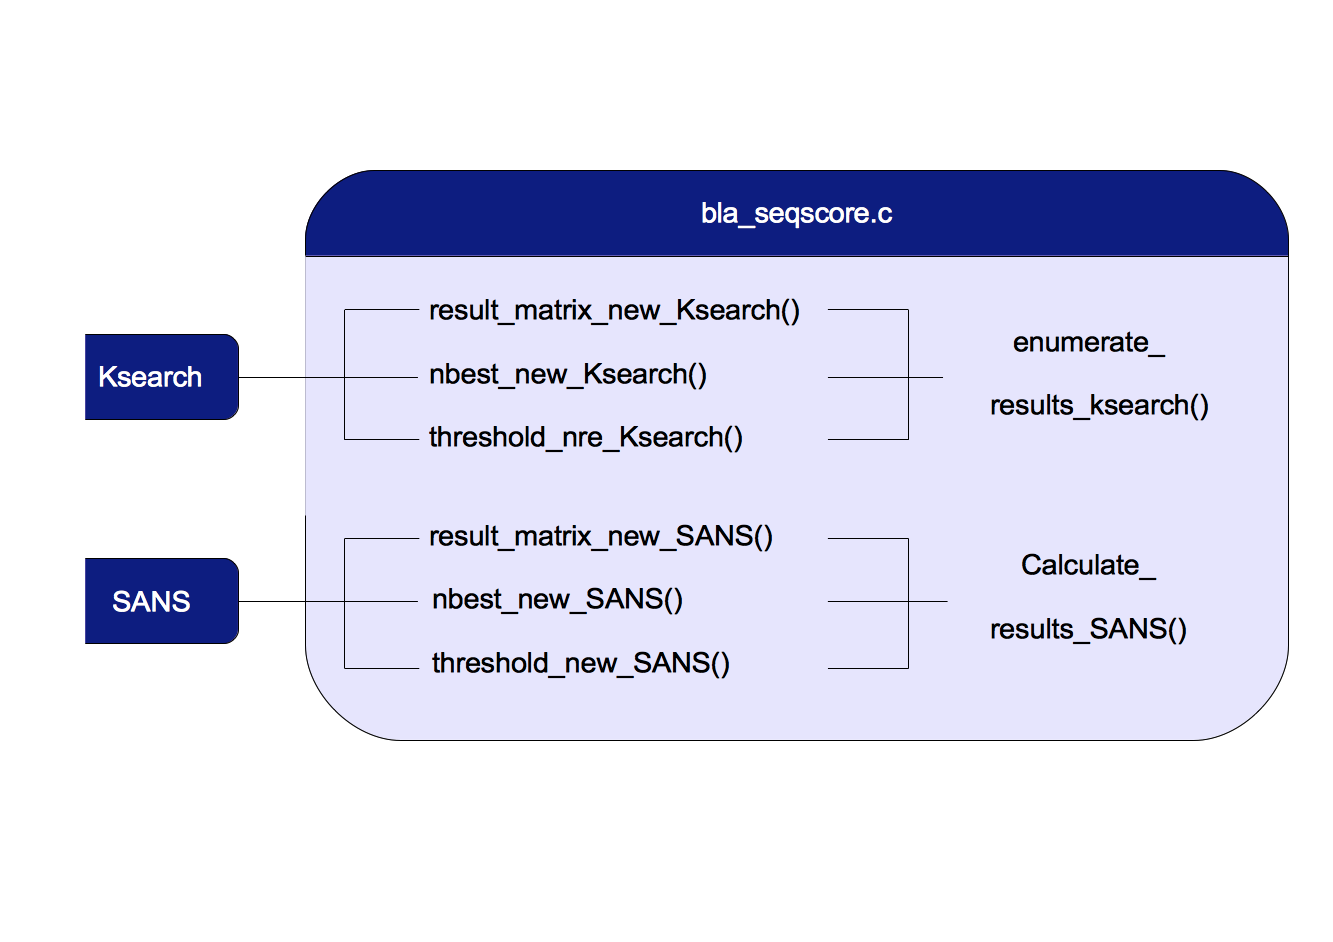
\includegraphics[width = \linewidth]{img/dia2}
    \caption{Struktur der \emph{bla\_seqscore.c}. Pro von Außen aufrufendem Tool sind drei Konstruktoren vorhanden, die jedoch jeweils wieder die
    selbe Berechnungsfunktion ausführen.}
    \label{seqsc}
  \end{figure}
\end{center}

Pro Algorithmus wurde eine tatsächliche Berechnungsfunktion implementiert. Auf diese wird aus den drei Ergebnisstruktur abhängigen Konstruktoren des jeweiligen
Algorithmus zugegriffen. Wir gehen zunächst auf den \emph{SANS} Algorithmus ein.

Da durch die unter Abschnitt \ref{sans} vorgestellte Berechnungsvorschrift der Score für ein Sequenzpaar erst bei der Terminierung des ALgorithmus
fest steht, muss für jeden \emph{SANS} Lauf die gesamte Ergebnismatrix der Dimension $|Q|\cdot|D|$ mitgeführt werden. Die Konstruktoren 
\emph{result\_matrix\_new\_sans()}, \emph{nbest\_new\_sans()} und  \emph{threshold\_new\_sans()} definieren also jeweils die Ergebnismatrix und allokieren
den entsprechenden Speicher und rufen dann die \emph{calculate\_results\_sans()} Funktion auf, die die Matrix füllt. Anschließend werden die Daten 
wiederum Konstruktorspezifisch aufbereitet. Der \emph{matrix}-Konstruktor wird also die gesamte Matrix, der \emph{nbest}-Konstruktor eine
Liste der $n$ besten Scores und der dazugehörigen Sequenzen und der \emph{treshold}-Konstruktor alle Sequenzpaare, deren Score über dem gegebenen
Schwellwert liegt, zurückgeben.

Wie in Abschnitt \ref{ksearch} ersichtlich, kann beim \emph{KSEARCH}-Algorithmus Speicherplatz gespart werden, da die Scores der Sequenzpaare
nacheinander ausgerechnet werden. Es muss also nur wenn der Benutzer die \emph{matrix}-Rückgabe gewünscht hat tatsächlich der Speicher für die
ganze Ergebnismatrix allokiert werden. Dies nutzen wir aus, indem die Konstruktoren \emph{result\_matrix\_new\_ksearch()}, \emph{nbest\_new\_ksearch()} 
und  \emph{threshold\_new\_ksearch()} eine ausgabespezifische Ergebnisstruktur erstellen und neben dieser Struktur auch eine Callback-Funktion an 
die \emph{enumerate\_results\_ksearch()} Funktion übergeben. Wie der Name der Funktion bereits anzeigt, berechnet die Funktion due \emph{KSEARCH}-Scores
sequenziell und ruft für jeden berechneten Score die übergebene Callback Funktion auf. Dieser wird auch die Ergebnisstruktur übergeben, so dass diese
der gewünschten Ausgabe entsprechend gefüllt werden kann. Abbildung \ref{kscallback} zeigt die Aufruf-Reihenfolge und die übergebenen Datenstrukturen am
Beispiel des \emph{result\_matrix\_new\_ksearch} Konstruktors.

\begin{center}
  \begin{figure}
    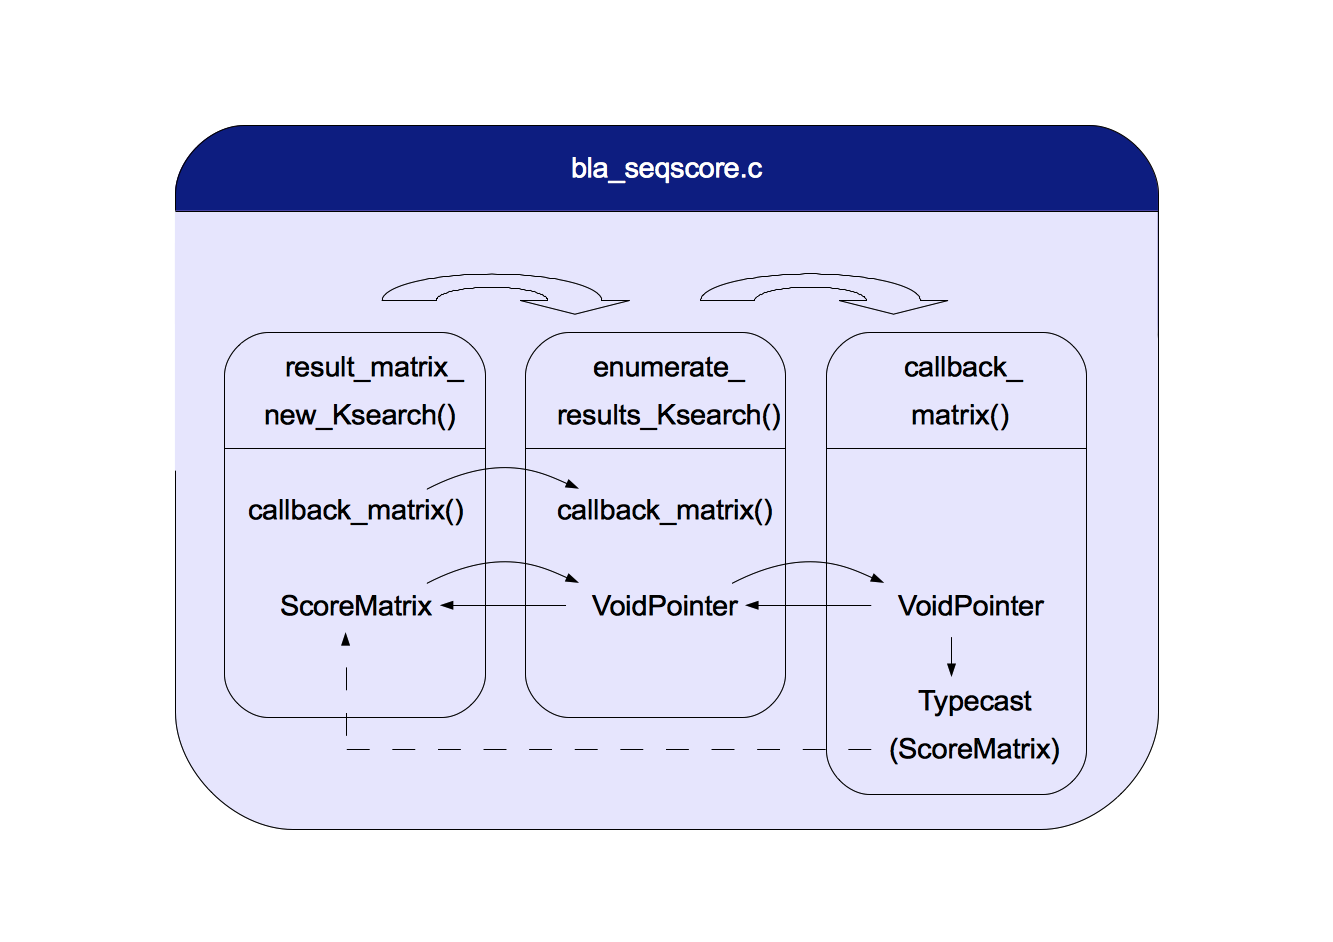
\includegraphics[width = \linewidth]{img/dia3}
    \caption{Aufruf-Reiehenfolge bei Aufruf des \emph{result\_matrix\_new\_ksearch} Konstruktor. Der Konstruktor übergibt der Funktion zur Score-Berechnung
      die Callback-Funktion \emph{callback\_matrix()} sowie die \emph{ScoreMatrix} als Ergebnisstruktur. Erst in der Callback-Funktion, die in der 
      Berechnungsfunktion aufgerufen wird, wird die Ergebnisstruktur wieder zu einer Matrix gecastet und befüllt.}
    \label{kscallback}
  \end{figure}
\end{center}

Für die \emph{matrix}-Option ist diese Rückgabestruktur ein einfaches zweidimensionales Array. Für die \emph{nbest} Option wurde eine in den genometools
bereits vorhandene Implementierung eines Red-Black-Trees als verkettete Liste genutzt. Diese kann schnell prüfen, ob ein neu generierter Score kleiner oder
grüßer als das bisher kleinste Element ist und entsprechend verfahren. Im Falle der \emph{threshold}-Option ist keine Ergebnisstruktur nötig,
da ein berechneter Score, der über dem gegebenen Schwellwert liegt, unmittelbar ausgegeben werden kann.

\section{Auswertung}

\end{document}
